\chapter{Methodology}


\section{Data set description}

The same data set as Wu et. al is used which is part of the publicly available 
benchmark data sets of MoleculeNet.\cite{wu2018moleculenet} This data set contains 
the measured solubility at $25^{\circ} C$ in $log(mol/L)$ for $1110$ compounds when duplicates 
are removed. Molecules are represented as a string using the simple molecular 
line entry system \big(SMILES\big).\cite{weininger1988smiles} 





\section{Architecture of the graph neural network model to predict water solubility}


Prediction of water solubility is achieved using the same RGCN model as Wu et. al.,
with the hyper parameters listed in \cref{tab:hyperparameters}. To obtain more 
robust predictions, ten models are trained, each with a different seed 
$(2023 + 10i, \text{ with } i \in \{1, 2, \dots, 10\})$, where the final 
prediction is then obtained by the average prediction over all models.


\begin{table}[h]
    \caption{ Hyper parameters from \protect\citen{wu2023chemistry} of an RGCN model to predict water solubility.}
    \label{tab:hyperparameters}
    \begin{center}
        \begin{tabular}{cc}
            \toprule
            \textbf{hyper parameter} & \textbf{value} \\
            \midrule
            RGCN layers & 2 \\
            RGCN hidden units & 256 \\
            RGCN dropout rate (each layer) & 0.5 \\
            MLP hidden units & 64 \\
            MLP dropout rate (each layer) & 0.1 \\ 
            Epochs & 500 \\
            Early stop & 30 \\
            \bottomrule
        \end{tabular}
    \end{center}
\end{table}


\begin{figure}[h]
    \centering 
    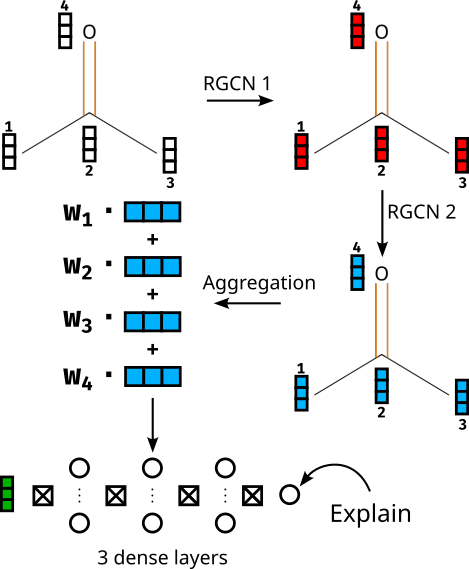
\includegraphics{../../data/images/RGCN_model.png}
\end{figure}
